\chapter{Background}
\label{background}

\section{Linear Algebra}

This section provides the minimum background knowledge of advanced concepts in the field of linear algebra.

\subsection{Unitary Operator}
\label{background:linear-algebra:unitary-operator}

If an operator is unitary if it satisfies the following conditions.

\begin{equation}
  U^{-1} = U^{\dagger}
\end{equation}

\begin{equation}
  UU^{\dagger} = U^{\dagger}U = I
\end{equation}

\section{Quantum Physics}

This section provide the fundamental knowledge of quantum physics, which will make readers feel familiar with the concept and notations that they will encounter throughout this thesis.

\subsection{Four Postulates}

This subsection introduces the basic principles, in other words, the postulates of quantum mechanics \cite{10.5555/1972505}.

\subsubsection{Postulate 1}

Associated with any isolated physical system is a complex vector space with inner product know as the \textit{state space} of the system.
The system is completely described by a \textit{state vector}, which is a unit vector in the system's state space.

\subsubsection{Postulate 2}

The evolution of a \textit{closed} quantum system is described by a \textit{unitary transformation}.
That is, the state $|\psi\rangle$ of the system at time $t_1$ is related to the state $|\psi'\rangle$ of the system $t_2$ by a unitary operator $U$ which depends only on the times $t_1$ and $t_2$.

\begin{equation}
  |\psi(t_2) \rangle = U|\psi(t_1)\rangle
\end{equation}


\subsubsection{Postulate 3}

Quantum measurements are described by a collection $\{M_m\}$ of \textit{measurement operators}.
These are operators acting on the space of the system being measured. The index $m$ refers to the measurement outcomes that may occur in the experiment.
If the state of the quantum system is $|\psi\rangle$ immediately before the measurement then the probability that result $m$ occurs is given by 
\begin{equation}
  p(m) = \langle \psi |M^{\dagger}_m M_m | \psi \rangle
\end{equation}


and the state of the system after the measurement is 

\begin{equation}
  \frac{M_m|\psi\rangle}{\langle \psi |M^{\dagger}_m M_m | \psi \rangle}
\end{equation}


The measurement operators satisfy the \textit{completeness equation}.
\begin{equation}
  \sum_m M^{\dagger}_m M_m = I
\end{equation}


The completeness equation expresses the fact that probability sum to one.
\begin{equation}
  1 = \sum_m p(m) = \sum_m \langle \psi |M^{\dagger}_m M_m | \psi \rangle
\end{equation}


\subsubsection{Postulate 4}

The state space of a composite physical system is the tensor product of the state space of the component physical systems. 
Moreover, if we have systems numbered 1 through $n$, and system number $i$ is prepared in the state $|\psi_i\rangle$, then the joint state of the total system is $|\psi_1\rangle \otimes |\psi_2\rangle \otimes \dots \otimes |\psi_n\rangle$.


\subsection{Pure State}

A pure state is the representation of quantum state of the whole system without the assumption of external noise.

\subsubsection{Definition}

A conventional computer uses a bit to represent a basic unit of information, which has the possible values 0 and 1. A basic unit of quantum information, on the other hand, is called a quantum bit (or \textbf{qubit} in short) wit possible values $|0\rangle$ and $|1\rangle$, each of which can be described in the form of a vector. 

For example  

\begin{equation}
  |0\rangle = \Big[
    \begin{array}{c}
    1 \\
    0 \\
    \end{array}
    \Big]
\end{equation}

\begin{equation}
  |1\rangle = \Big[
\begin{array}{c}
0 \\
1 \\
\end{array}
\Big]
\end{equation}


The state of a single qubit $|\psi\rangle$ can be described as follows.
\begin{equation}
  |\psi\rangle = \alpha |0\rangle + \beta |1\rangle \,(\alpha, \beta \in \mathbb{C}, |\alpha|^2+|\beta|^2=1).
\end{equation}

 After the operation called measurement, the quantum state would be collapsed into either 0 or 1.  The measurement probability of 0 is $|\alpha|^2$ and that of 1 is $|\beta|^2$. In other words, a single qubit can take both states probabilistically at the same time.  
 
 For instance, a qubit can be 
 
\begin{equation}
	|\psi\rangle = \frac{1}{\sqrt{2}}|0\rangle + \frac{1}{\sqrt{2}}|1\rangle \tag{1}
\end{equation}

 whose measurement probability of 0 and 1 is 50\% and 50\% respectively.

\subsubsection{Bloch Sphere}
Because $|\alpha|^2 + |\beta|^2 = 1$, the notation of a single qubit state can be represented like this.

\begin{equation}
|\psi\rangle = e^{i\gamma} (\cos{\frac{\theta}{2}} + e^{i\phi} \sin{\frac{\theta}{2}}) (\gamma, \phi, \theta \in \mathbb{R})
\end{equation}.

Because $e^{i\gamma}$ is just a global phase, it can be ignored because it does not change the measurement probability of each state and therefore it does not cause any observable effect.

\begin{equation}
 |\psi\rangle =  \cos{\frac{\theta}{2}} + e^{i\phi} \sin{\frac{\theta}{2}} (\phi, \theta \in \mathbb{C})
\end{equation}

Because the equation above has two parameters, any pure single qubit state can be considered as a point on the surface of a sphere and its geometric representation is called the \textbf{Bloch sphere}.

\begin{figure}[ht]
  \centering
  \tikz{
    \tikzstyle{st}=[lightgray, fill, fill opacity=0.2];
    \coordinate(o)at(0,0); 
    \draw(o)circle(2cm); 
    \draw[fill](o)circle(1.5pt);%origin
    \draw[st](o)--(56.7:0.4)arc(56.7:90.:0.4)--cycle;%theta angle
    \draw(0.18,0.6)node{$\theta$};
    \draw[st](o)--(-135.7:0.4)arc(-135.7:-33.2:0.4)--cycle;%varphi angle
    \draw(0.14,-0.58)node{$\varphi$};
    \draw[->](o)--(-0.81,-0.79) node[above left]{\ $x$};%x
    \draw[->](o)--(2,0)node[right]{$y$};%y
    \draw[->](o)--(0,2)node[below right]{$z$}node[above]{\ $\ket{0}$};%z |0>
    \draw[rotate around={0.:(0.,0.)},dashed](0,0)ellipse(2cm and 0.9cm);%ellipse
    \draw[thick,->](o)--(0.70,1.07)node[above]{\ $\ket{\psi}$};%state vector
    \draw[densely dotted,->](o)--(0,-2)node[below]{\ $\ket{1}$};%-z |1>
    \draw[dotted](o)--(0.7,-0.46)--(0.7,1);%triangle
  }
    
\newpage
\caption{Bloch Sphere}
\end{figure}

\subsubsection{Multi-Qubit State}
  The quantum state for multi-qubits is a \textbf{tensor product} of a state vector of each qubit.  The general notation of a two qubit state is
  
\begin{align}
    |\psi\rangle & = (\alpha |0\rangle + \beta |1\rangle) \otimes  (\gamma |0\rangle + \delta |1\rangle) \nonumber\\
    & = \alpha \gamma |00\rangle + \alpha \delta |01\rangle + \beta \gamma |10\rangle + \beta \delta |11\rangle \nonumber\\ 
   & (\alpha, \beta, \gamma, \delta \in \mathbb{C}, |\alpha|^2+|\beta|^2+|\gamma|^2+|\delta|^2=1)
\end{align}
  
  For example, the state $|00\rangle$ is equal to 
  
\begin{equation}
  \left[
\begin{array}{c}
1 \\
0 \\
\end{array}
\right]
\otimes
 \left[
\begin{array}{c}
1 \\
0 \\
\end{array}
\right]
= \left[
\begin{array}{c}
1 \\
0 \\
0 \\
0 \\
\end{array}
\right]
\end{equation}.

 However, some quantum states such as
 
 \begin{equation}
 	|\psi\rangle = \frac{1}{\sqrt{2}}|00\rangle + \frac{1}{\sqrt{2}}|11\rangle
 \end{equation}
 
 cannot be decomposed into independent quantum state of each qubit.  These special quantum states are called \textbf{entangled} states.

 \subsubsection{Measurement}
Quantum measurement can be described by using a group of measurement operators $\{M_m\}$
($m$ is the measurement result that is expected to get). It is worth noting the fact that a measurement operator is not unitary.
 If the quantum state before measurement is $|\psi\rangle$, the measurement probability of value $m$ is 
 \begin{equation}
  p(m) = \langle \psi|M^{\dagger}_m M_m|\psi\rangle
 \end{equation}


 The quantum state after the measurement is 
 \begin{equation}
  \frac{M_m|\psi\rangle}{\sqrt{\langle \psi|M^{\dagger}_m M_m|\psi\rangle}}
 \end{equation}


The measurement operators satisfy the completeness equation
\begin{equation}
  \sum_{m} M^{\dagger}_m M_m = I
\end{equation}


Also, the sum of the measurement probability of each possible measurement outcome is equal to one.
\begin{equation}
  \sum_{m} p(m) = \langle \psi|\sum_{m} M^{\dagger}_m M_m|\psi\rangle = 1
\end{equation}

 \subsection{Mixed State}
 %TODO: Add general principles of density metrics and their proofs
%TODO: ADD proof that a density matrix is positive semidefinite

 A mixed state is another representation of quantum state in more general cases, such as the presense of physical error.
A mixed state is described in the form of a matrix which is called a density matrix. 

\subsubsection{Definition}

The density matrix of this system $\rho$ is described by 

\begin{equation}
  \rho = \sum_i p_i |\psi_i\rangle\langle\psi_i|.
\end{equation}

\subsubsection{Evolution}

The quantum system after applying a unitary operator $U$ is
\begin{equation}
  \rho = \sum_i p_i |\psi_i\rangle\langle\psi_i| \xrightarrow{U} \sum_i p_i U|\psi_i\rangle\langle\psi_i|U^{\dagger}
\end{equation}
It is worth noting that a unitary operation on a single qubit is equivalent to the rotation of a vector on the surface of the Bloch sphere.
\subsubsection{Measurement}

Suppose one performs measurement on a quantum state $|\psi_i\rangle$ using a measurement operator $M_m$. 

Then, the measurement probability of $m$ is 
\begin{equation}
  p(m|i) = \langle\psi_i|M^{\dagger}_m M_m|\psi_i\rangle = tr(M^{\dagger}_m M_m|\psi_i\rangle\langle\psi_i|)
\end{equation}

The measurement probability of $m$ from the collection of states $\{|\psi_i\rangle\}$ is 
\begin{equation}
  \begin{split}
    p(m) &= \sum_i p_i p(m|i) \\ 
    &= \sum_i p_i \langle\psi_i|M^{\dagger}_m M_m|\psi_i\rangle \\
    &= \sum_i p_i \tr(M^{\dagger}_m M_m|\psi_i\rangle\langle\psi_i|) \\
    &= \tr(M^{\dagger}_m M_m \rho).
  \end{split}
\end{equation}

The quantum state after the measuring $|\psi_i\rangle$ is 
\begin{equation}
  |\psi^m_i\rangle = \frac{M_m|\psi^m_i\rangle}{\sqrt{\langle \psi^m_i|M^{\dagger}_m M_m|\psi^m_i\rangle}}.
\end{equation}

The corresponding density matrix is
\begin{equation}
  \begin{split}
    \rho_m = \sum_i p(i|m)|\psi^m_i\rangle\langle\psi^m_i| = \sum_i p(i|m)\frac{M_m|\psi_i\rangle\langle\psi_i|M^{\dagger}_m}{\sqrt{\langle \psi^m_i|M^{\dagger}_m M_m|\psi^m_i\rangle}}
  \end{split}
\end{equation}

\begin{equation}
  \begin{split}
    p(i|m) &= \frac{p(m, i)}{p(m)} = \frac{p(m|i)p_i}{p(m)} \\
    &= \frac{\tr(M^{\dagger}_m M_m \rho) p_i}{\tr(M^{\dagger}_m M_m \rho)} \\
    &= p_i.
  \end{split}
\end{equation}

Therefore, the state can also be described by the equation
\begin{equation}
  \begin{split}
    \rho_m &= \sum_i p_i \frac{M_m|\psi_i\rangle\langle\psi_i|M^{\dagger}_m}{\tr(M^{\dagger}_m M_m \rho)} \\
    &= \frac{M_m \rho M^{\dagger}_m}{\tr(M^{\dagger}_m M_m \rho)}.
  \end{split}
\end{equation}


 \subsection{Fidelity}
  %TODO: Add proof that the square root of density matrix exists in the appendix
  %TODO: Mention the fact above in this subsection.

 Fidelity is one of a distance measure between two quantum state. the fidelity of quantum state $\rho$ and $\sigma$ is
 \begin{equation}
  \begin{split}
    F(\rho, \sigma) &= \tr{\sqrt{\rho^{\frac{1}{2}}\sigma\rho^{\frac{1}{2}}}} \\
  \end{split}
\end{equation}

The fidelity between these two states would be
\begin{equation}
  \begin{split}
    F(\rho, \sigma) &= \tr{\sqrt{\sum_i r_i s_i |i\rangle\langle i|}} \\
    &= \tr(\sum_i \sqrt{r_i s_i} |i\rangle\langle i|) \\
    &= \sum_i \sqrt{r_i s_i}
  \end{split}
\end{equation}

The fidelity between a pure state $|\psi\rangle$ and a mixed state $\rho$ is 
\begin{equation}
  \begin{split}
    F(\psi, \rho) &= \tr{\sqrt{\langle\psi|\rho|\psi\rangle|\psi\rangle\langle\psi|}} \\
    &= \sqrt{\langle\psi|\rho|\psi\rangle}
  \end{split}
\end{equation}

\section{Quantum Operations}

Operators of quantum gates are unitary, while the one of the measurement operation is non-unitary.
The definition of a unitary operator is described in \ref{background:linear-algebra:unitary-operator}
\subsection{I Gate}

The I gate is equal to the 2 $\times$ 2 identity matrix, which is 

\begin{equation}
I = \begin{bmatrix}
1 & 0 \\
0 & 1 \\
\end{bmatrix}
\end{equation}.

For example,

\begin{equation}
 I|0\rangle = \begin{bmatrix}
1 & 0 \\
0 & 1 \\
\end{bmatrix} 
\left[
\begin{array}{c}
1 \\
0 \\
\end{array}
\right]
= \left[
\begin{array}{c}
1 \\
0 \\
\end{array}
\right]
= |0\rangle
\end{equation}

\begin{equation}
I|1\rangle = \begin{bmatrix}
1 & 0 \\
0 & 1 \\
\end{bmatrix} 
\left[
\begin{array}{c}
0 \\
1  \\
\end{array}
\right]
= \left[
\begin{array}{c}
0 \\
1 \\
\end{array}
\right]
= |1\rangle
\end{equation}.

\subsection{X Gate}
\subsubsection{X gate}

The X gate flips the logical value of a qubit.

\begin{equation}
X = \begin{bmatrix}
0 & 1 \\
1 & 0 \\
\end{bmatrix}
\end{equation}.

For example,
\begin{equation}
X|0\rangle = \begin{bmatrix}
0 & 1 \\
1 & 0 \\
\end{bmatrix} 
\left[
\begin{array}{c}
1 \\
0 \\
\end{array}
\right]
= \left[
\begin{array}{c}
0 \\
1 \\
\end{array}
\right]
= |1\rangle
\end{equation}

\begin{equation}
 X|1\rangle = \begin{bmatrix}
0 & 1 \\
1 & 0 \\
\end{bmatrix} 
\left[
\begin{array}{c}
0 \\
1  \\
\end{array}
\right]
= \left[
\begin{array}{c}
1 \\
0 \\
\end{array}
\right]
= |0\rangle
\end{equation}.

\subsection{Y Gate}

The Y gate flips the logical value of a qubit and adds an imaginary phase.

\begin{equation}
 Y = \begin{bmatrix}
0 & -i \\
i & 0 \\
\end{bmatrix}
\end{equation}.

For example,
\begin{equation}
Y|0\rangle = \begin{bmatrix}
0 & -i \\
i & 0 \\
\end{bmatrix} 
\left[
\begin{array}{c}
1 \\
0 \\
\end{array}
\right]
= \left[
\begin{array}{c}
0 \\
i \\
\end{array}
\right]
= i|1\rangle
\end{equation}

\begin{equation}
Y|1\rangle = \begin{bmatrix}
0 & -i \\
i & 0 \\
\end{bmatrix} 
\left[
\begin{array}{c}
0 \\
1  \\
\end{array}
\right]
= \left[
\begin{array}{c}
-i \\
0 \\
\end{array}
\right]
= -i|0\rangle
\end{equation}.

\subsection{Z Gate}
The Z gate flips the phase of $ |1\rangle$

\begin{equation}
 Z = \begin{bmatrix}
1 & 0 \\
0 & -1 \\
\end{bmatrix}
\end{equation}.

For example,
\begin{equation}
 Z|0\rangle = \begin{bmatrix}
1 & 0 \\
0 & -1 \\
\end{bmatrix} 
\left[
\begin{array}{c}
1 \\
0 \\
\end{array}
\right]
= \left[
\begin{array}{c}
1 \\
0 \\
\end{array}
\right]
= |0\rangle
\end{equation}

\begin{equation}
Z|1\rangle = \begin{bmatrix}
1 & 0 \\
0 & -1 \\
\end{bmatrix} 
\left[
\begin{array}{c}
0 \\
1  \\
\end{array}
\right]
= \left[
\begin{array}{c}
0 \\
-1 \\
\end{array}
\right]
= -|1\rangle
\end{equation}.

\subsection{H Gate}
The Hadamard or, the H gate creates superposition.
\begin{equation}
 H = \frac{1}{\sqrt{2}}\begin{bmatrix}
1 & 1\\
1 & -1 \\
\end{bmatrix}
\end{equation}.

For example,
\begin{equation}
H|0\rangle = \frac{1}{\sqrt{2}}\begin{bmatrix}
1 & 1\\
1 & -1 \\
\end{bmatrix}\left[
\begin{array}{c}
1 \\
0 \\
\end{array}
\right]
= \frac{1}{\sqrt{2}} \left[
\begin{array}{c}
1 \\
1 \\
\end{array}
\right]
= \frac{1}{\sqrt{2}} (|0\rangle + |1\rangle)
\end{equation}

\begin{equation}
H|1\rangle = \begin{bmatrix}
1 & 1\\
1 & -1 \\
\end{bmatrix} 
\left[
\begin{array}{c}
0 \\
1  \\
\end{array}
\right]
= \frac{1}{\sqrt{2}} \left[
\begin{array}{c}
1 \\
-1 \\
\end{array}
\right]
=\frac{1}{\sqrt{2}} (|0\rangle - |1\rangle)
\end{equation}.

\subsection{Rotation Gate}

Rotation gates are quantum gates that represent rotation through an arbitrary angle $\theta$ with respect to one of the x, y, z-axes of the Bloch sphere.

\begin{equation}
  R_x(\theta) = e^{-iX\theta/2} = \cos \frac{\theta}{2}I - i \sin\frac{\theta}{2}X = \begin{bmatrix}
    \cos \frac{\theta}{2} & -i \sin \frac{\theta}{2} \\
    -i \sin \frac{\theta}{2} & \cos \frac{\theta}{2} \\
    \end{bmatrix} 
\end{equation}

\begin{equation}
  R_y(\theta) = e^{-iY\theta/2} = \cos \frac{\theta}{2}I - i \sin\frac{\theta}{2}Y = \begin{bmatrix}
    \cos \frac{\theta}{2} & -\sin \frac{\theta}{2} \\
    \sin \frac{\theta}{2} & \cos \frac{\theta}{2} \\
    \end{bmatrix} 
\end{equation}

\begin{equation}
  R_z(\theta) = e^{-iZ\theta/2} = \cos \frac{\theta}{2}I - i \sin\frac{\theta}{2}Z = \begin{bmatrix}
    e^{-i \frac{\theta}{2}} & 0 \\
    0 & e^{i \frac{\theta}{2}} \\
    \end{bmatrix} 
\end{equation}

\subsection{General One Qubit Gate}

An arbitrary single qubit operation $U$ can be decomposed into three rotation gates with an additional phase $\alpha$.

\begin{equation}
 U = e^{i \alpha}R_z(\beta)R_y(\gamma)R_z(\delta) = \begin{bmatrix}
    e^{i (\alpha-\beta/2-\gamma/2)\cos\frac{\delta}{2}} & e^{i (\alpha-\beta/2+\gamma/2)\sin\frac{\delta}{2}}  \\
    e^{i (\alpha+\beta/2-\gamma/2)\sin\frac{\delta}{2}}  & e^{i (\alpha+\beta/2+\gamma/2)\cos\frac{\delta}{2}}  \\
    \end{bmatrix} 
\end{equation}

\subsection{Controlled-NOT Gate}
A CNOT gate involves two qubits, one is called \textbf{the controll qubit} and the other is called \textbf{target qubit}.  If the control qubit is 1, the bit value of the target qubit is flipped.

\begin{equation}
CNOT = \begin{bmatrix}
1 & 0 & 0 & 0 \\
0 & 1 & 0 & 0 \\
0 & 0 & 0 & 1 \\
0 & 0 & 1 & 0 \\
\end{bmatrix}
\end{equation}.

For example,
\begin{equation}
CNOT_{0,1}|10\rangle = 
\begin{bmatrix}
1 & 0 & 0 & 0 \\
0 & 1 & 0 & 0 \\
0 & 0 & 0 & 1 \\
0 & 0 & 1 & 0 \\
\end{bmatrix}
 \left[
\begin{array}{c}
0 \\
0 \\
1 \\
0 \\
\end{array}
\right]
=  \left[
\begin{array}{c}
0 \\
0 \\
0 \\
1 \\
\end{array}
\right] 
= |11\rangle 
\end{equation}

\begin{equation}
CNOT_{0,1}|11\rangle = 
\begin{bmatrix}
1 & 0 & 0 & 0 \\
0 & 1 & 0 & 0 \\
0 & 0 & 0 & 1 \\
0 & 0 & 1 & 0 \\
\end{bmatrix}
 \left[
\begin{array}{c}
0 \\
0 \\
0 \\
1 \\
\end{array}
\right]
=  \left[
\begin{array}{c}
0 \\
0 \\
1 \\
0 \\
\end{array}
\right] 
= |10\rangle 
\end{equation}.

\subsection{Controlled-Z Gate}
A CZ gate involves two qubits, one is called \textbf{the control qubit} and the other is called \textbf{target qubit}.  If the control qubit is 1, the Z gate is applied to the target qubit.

\begin{equation}
CZ = \begin{bmatrix}
1 & 0 & 0 & 0 \\
0 & 1 & 0 & 0 \\
0 & 0 & 1 & 0 \\
0 & 0 & 0 & -1 \\
\end{bmatrix}
\end{equation}.

For example,
\begin{equation}
CZ_{0,1}|10\rangle = 
\begin{bmatrix}
1 & 0 & 0 & 0 \\
0 & 1 & 0 & 0 \\
0 & 0 & 1 & 0 \\
0 & 0 & 0 & -1 \\
\end{bmatrix}
 \left[
\begin{array}{c}
0 \\
0 \\
1 \\
0 \\
\end{array}
\right]
=  \left[
\begin{array}{c}
0 \\
0 \\
1 \\
0 \\
\end{array}
\right] 
= |10\rangle 
\end{equation}

\begin{equation}
CZ_{0,1}|11\rangle = 
\begin{bmatrix}
  1 & 0 & 0 & 0 \\
  0 & 1 & 0 & 0 \\
  0 & 0 & 1 & 0 \\
  0 & 0 & 0 & -1 \\
  \end{bmatrix}
 \left[
\begin{array}{c}
0 \\
0 \\
0 \\
1 \\
\end{array}
\right]
=  \left[
\begin{array}{c}
0 \\
0 \\
0 \\
-1 \\
\end{array}
\right] 
= -|11\rangle 
\end{equation}.


% TODO: Add general properties of density operators

\section{Quantum Circuit}
Fig \ref{background:example-circuit} is an example of a quantum circuit.

\begin{figure}[ht]
  \begin{center}
    \begin{tikzpicture}
    \begin{yquant}
      qubit {$\ket{\reg_{\idx}}$} a[3];
      h a[0];
      h a[1];
      h a[2];
      cnot a[0] | a[1];
      x a[2];	
      y a[0];	 
      cnot a[1] | a[2]; 
      measure a[0-2];					 
     \end{yquant}
  \end{tikzpicture}
\caption{A example of a quantum circuit}
\end{center}
\label{background:example-circuit}
\end{figure}

Each horizontal line represents each qubit and the square boxes that contain letters mean single quantum gates.  The sign which involves a vertical line means a CNOT gate, and the box on the most right side indicates measurement. 

\section{Quantum Entanglement}

Quantum entanglement is a special type of quantum state that cannot be described in the form of tensor product of the state of each particle.

\subsection{Bell Pair}
The entangled states between two qubits are called Bell pairs or EPR pairs \cite{PhysRev.47.777}, and each of four states has a special notation.

\begin{equation}
  |\Phi^+\rangle = \frac{|00\rangle + |11\rangle}{\sqrt{2}}
  \end{equation}
  
  \begin{equation}
 |\Phi^-\rangle = \frac{|00\rangle - |11\rangle}{\sqrt{2}}
 \end{equation}
 
 \begin{equation}
 |\Psi^+\rangle = \frac{|01\rangle + |10\rangle}{\sqrt{2}}
 \end{equation}
 
 \begin{equation}
  |\Psi^-\rangle = \frac{|01\rangle - |10\rangle}{\sqrt{2}}
  \end{equation}.

\subsection{Multipartite Entanglement}
There are cases that more than two qubits are entangled. One such state is called the Greenberger-Horne-Zeilinger state or GHZ state.
The GHZ state is the only one of the infinite number of possible entangled states.

\ref{background:three-qubits} is the braket notation of the GHZ state that involves three qubits.
\begin{equation}
  |GHZ\rangle = \frac{|000\rangle + |111\rangle}{\sqrt{2}}
  \label{background:three-qubits}
\end{equation}.

In the general case, the braket notation of the GHZ state of N qubits is the following.
\begin{equation}
  |GHZ\rangle = \frac{|0\rangle^{\otimes N} + |1\rangle^{\otimes N}}{\sqrt{2}}
\end{equation}.

\subsection{Graph State}

A graph state is a particular multipartite entangled state. 
Given a particular graph $G(V, E)$, V indicates the collection of vertices and $E$ indicates the collection of edges.
The associated graph state $|G\rangle$ would be represented as 
\begin{equation}
  |G\rangle = \prod_{(a,b) \in E} CZ_{a,b} |+\rangle
\end{equation}.

First, all the qubits are initialized as $|+ \rangle$ states and then Controlled-Z gates are applied to each pair of qubits that is represented by an edge.
A graph state is also known as the initial state for measurement-based quantum computation (MBQC) \cite{PhysRevLett.86.5188}. 

\subsection{Bell State Measurement}
Bell state measurement is a special type of quantum measurement that determines which Bell pair the given two qubit entangled state is \cite{PhysRevA.59.3295}.
If the state is a superposition of Bell states, the system is projected into one of them probabilistically.

\begin{figure}[ht]
  \begin{center}
    \begin{tikzpicture}
    \begin{yquant}
      qubit {$\ket{\reg_{\idx}}$} a[2];
      cnot a[0] | a[1];
      h a[0];	 
      measure a[0-1];					 
     \end{yquant}
  \end{tikzpicture}
\caption{Quantum circuit for Bell state measurement}
\end{center}
\end{figure}

\begin{table}[ht]
  \begin{center}
    \begin{tabular}{|c|c|} \hline
      Measurement results & Bell state \\ \hline \cline{1-2}
      00 &  $|\Phi^+\rangle$ \\ \cline{1-2}
      01 & $|\Phi^-\rangle$ \\  \cline{1-2}
      10 &  $|\Psi^+\rangle$ \\ \cline{1-2}
      11 & $|\Psi^-\rangle$ \\  \hline  \cline{1-2}
    \end{tabular}
    \caption{A table of correspondence between measurement result and Bell pair}
  \end{center}
\end{table}

\subsection{Quantum Teleportation}

Unlike classical communication, quantum states cannot be just copied and transmit to other nodes due to the no-cloning theorem, which forbids duplication of any quantum state.  

However, a method called quantum teleportation was proposed \cite{PhysRevLett.70.1895}, which overcomes the restriction and allows sender to transmit single qubit state to a distant location. 
 		
This method requires both the single qubit state and a new Bell pair. 
After applying a CNOT gate and an H gate between the single qubit and the first qubit of the Bell pair, the sender has to measure both qubits and send those measurement results over the classical network.  
Then, the receiver gets those measurement results and apply some quantum gates if the measurement results of corresponding qubits on the sender's side are 1, in order to correct on the quantum state on the receiver's side.

This protocol has been experimentally demonstrated over up to 1,400 km \cite{ren2017ground}.

Fig \ref{fig:quantum-teleporatation} is the figure of the quantum circuit that performs quantum teleportation for a single qubit information \cite{9023997}.

\begin{figure}[ht]
  	\begin{center}
  		\begin{tikzpicture}
			\begin{yquant}
	 			qubit {$\ket{\reg_{\idx}}$} a[2];
	 			qubit {$\ket{\reg_{\idx}}$} b[1];
	 			h a[1];
        cnot b[0] | a[1];
	 			cnot a[1] | a[0];
        h a[0];	 
        measure a[0-1];	
        z b[0] | a[0];	
        x b[0] | a[1];				 
 			\end{yquant}
		\end{tikzpicture}
	\caption{Quantum circuit for quantum teleportation}
  \label{fig:quantum-teleporatation}
	\end{center}
\end{figure}

\newpage

\subsection{Entanglement Swapping}

Entanglement swapping is the method to extend quantum entanglement by performing joint measurement on several quantum entanglement \cite{zukowski1993event}.

For example, assume Alice has a single qubit, Bob has two qubits, and Charlie has one qubit. Then, there are Bell pairs between Alice's qubit and Bob's first qubit, and Bob's second qubit and Charlie's qubit, respectively.
If Bob performs Bell state measurement on both of his qubits, Alice's qubit and Charlie's qubit are eventually entangled, even though they have not interacted with each other.
This can be also seen as the teleportation of a Bell pair by sending one of its particles. 

This method has been experimentally demonstrated by using polarization photon qubits in free space \cite{PhysRevLett.80.3891}, in optical fiber \cite{PhysRevA.71.050302}, and even using continuous variables \cite{jia2004experimental}.

\ref{background:entanglement-swapping} is the figure of quantum circuit to perform entanglement swapping \cite{9803043}.

\begin{figure}[ht]
  \begin{center}
    \begin{tikzpicture}
    \begin{yquant}
       qubit {$\ket{\reg_{\idx}}$} a[1];
       qubit {$\ket{\reg_{\idx}}$} b[2];
      qubit {$\ket{\reg_{\idx}}$} c[1];
       h a[0];
      h c[0];
       cnot b[0] | a[0];
       cnot b[1] | c[0];
      cnot b[1] | b[0];
      h b[0];	 
      measure b[0-1];	
      z a[0] | b[0];	
      x c[0] | b[1];		 
     \end{yquant}
  \end{tikzpicture}
\caption{Quantum circuit for entanglement swapping}
\end{center}
\label{background:entanglement-swapping}
\end{figure}

\subsection{Entanglement Purification}

Entanglement purification \cite{PhysRevA.53.2046} is a scheme to generate a set of quantum entanglements with higher fidelities from a larger set of imperfect quantum entanglements, local quantum operations, and classical communications.
This procedure is also called entanglement distillation, or quantum concatenation. This section presents an example of entanglement purification that generates a single Bell pair with higher fidelity from two of those with less fidelity.

This protocol has been experimentally demonstrated using photons \cite{Yan:21}, atoms \cite{179436} and electron-spin qubits \cite{kalb2017entanglement}.


Assume Alice and Bob are supposed to share $|\Phi^+\rangle$, which is one of the Bell pairs. However, the state would be converted to the following mixed state due to the noisy nature of a quantum channel.
\begin{equation}
  \rho_{AB} = P_{\Phi^+}|\Phi^+\rangle\langle\Phi^+| + P_{\Phi^-}|\Phi^-\rangle\langle\Phi^-| + P_{\Psi^+}|\Psi^+\rangle\langle\Psi^+| + P_{\Psi^-}|\Psi^-\rangle\langle\Psi^-|
\end{equation}

\begin{equation}
  \sum_{s \in \{\Phi^+, \Phi^-, \Psi^+, \Psi^- \}} P_{s} = 1
\end{equation}


Any mixed state might be converted to a Werner state by applying Pauli operations and $\frac{\pi}{2}$ operations, so Alice and Bob can obtain the following state.
\begin{equation}
  \rho^{'}_{AB} = F|\Phi^+\rangle\langle\Phi^+| + \frac{1-F}{3}(|\Phi^-\rangle\langle\Phi^-| + |\Psi^+\rangle\langle\Psi^+| + |\Psi^-\rangle\langle\Psi^-|)
\end{equation}

Fig \ref{background:werner-state} is the quantum circuit to prepare a Werner state.

\begin{figure}[H]
  \centerline{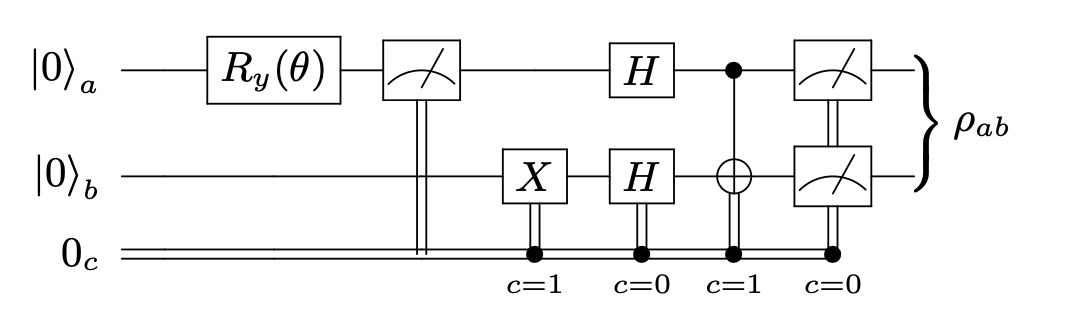
\includegraphics[width=0.8\columnwidth]{images/circuit_werner_state.png}}
  \caption{The figure of the circuit for entanglement purification \cite{riedel2021bell}}
  \label{background:werner-state}
\end{figure}


Two noisy Bell pairs are required for entanglement purification. One of the Bell pair $\rho^{'}_{a_1 b_1}$ is called the source Bell pair, which may be purified, and the other one $\rho^{'}_{a_2 b_2}$  is the called target Bell pair, which is going to be measured. 
Then, Alice and Bob perform CNOT operations between $a_1$ and $a_2$, and $b_1$ and $b_2$, respectively.
After that, they measure $a_2$ and $b_2$ respectively, which is the qubit on the target Bell pair on their side and exchange the measurement results. 
If their measurement results match, the purification is successful, while they have to discard the source Bell pair and try again if those results do not match.

The quantum state after measuring the target Bell pair, is

\begin{align}
\rho^{'}_{ab} = \frac{1}{N} \big[ F^2 + \frac{1}{9}\big(1-F \big)^2\big]|\Phi^+\rangle\langle\Phi^+| + \frac{2F(1-F)}{3N}|\Phi^-\rangle\langle\Phi^-| + \frac{2(1-F)^2}{9N}(|\Psi^+\rangle\langle\Psi^+| + |\Psi^-\rangle\langle\Psi^-|) \nonumber\\
(N = F^2 + \frac{2F(1-F)}{3} + \frac{2(1-F)^2}{9})
\end{align}

The purification becomes successful if F  $> \frac{1}{2}$. The readers can refer to more detailed calculation in the Appendix\ref{appendix:purification}

\section{Quantum Networking}

This section explains the important concepts of quantum networking.

\subsection{Quantum Node}

Quantum nodes are the nodes on a quantum network, which can be categorized into one of the following three categories, which was discussed in \cite{van2022quantum}

\subsubsection{End nodes}

\textbf{MEAS} measures the photons it receives. Although its functionality seems to be pretty limited, a pair of this type of node can perform quantum key distribution. In addition, a single node can be used as a terminal for blind quantum computation.

\textbf{COMP} represents quantum processor.  This node also has the functionality of measuring qubits and also storing them in quantum memories.

\textbf{SENS} has sensing functionality by using quantum entanglement, which can be used for clock synchronization and a reference frame for interferometry. 

\subsubsection{Quantum repeaters and routers}

\textbf{REP1} plays the role of the 1st generation quantum repeater. It performs entanglement swapping and improves the fidelity of Bell pair by purification.
The detail of each generation of quantum repeater network will be discussed in the later section.

\textbf{REP2} plays the role of the 2nd generation quantum repeater. It performs entanglement swapping and perform quantum error correction on logical qubits composed of several physical qubits.

\textbf{RTR} behaves as the border between two different networks and also involves rewriting the given RuleSets into either 1st generation protocol and 2nd generation protocol based on what the network assumes.

\subsubsection{Support nodes}

\textbf{EPPS}, which stands for an entangled photon pair source, performs spontaneous parametric down conversion (SPDC).
It creates pairs of entangled photons and send them to link end points. This node is used in terrestrial links or in satellite, which emits photons to telescopes on the ground.

\textbf{BSA} or Bell State Analyzer, generates a entangled state between two quantum memories by swapping two different entanglements between a single quantum memory and a single photon.
The success probability of entanglement swapping with linear optics scheme does not exceed 50\%.

\textbf{RGSS} generates multipartite photonic entangled state for memoryless quantum network. It sends each half of the generated repeater graph state to the neighboring nodes.
The photons are measured at link end nodes.

\textbf{ABSA} performs both a single-photon measurement and two-photon measurements and their measurement basis changes based on previous measurement outcomes, logical encoding and the structure of repeater graph states.

\textbf{OSW} plays a role of optical switches and can exist independently or as a part of the type of nodes that are mentioned above.
It switches photons from incoming links to outgoing ones.
